%%%%%%%%%%%%%%%%%%%%%%% Boundary-Layer Meteorology 2019 Template %%%%%%%%%%%%%%%%%%%%%%%%%


\begin{filecontents*}{example.eps}
gsave
newpath
  20 20 moveto
  20 220 lineto
  220 220 lineto
  220 20 lineto
closepath
2 setlinewidth
gsave
  .4 setgray fill
grestore
stroke
grestore
\end{filecontents*}

\RequirePackage{fix-cm}
\documentclass[smallextended]{svjour3}       
\smartqed  
\usepackage{appendix}
\usepackage{amsmath}
\usepackage{graphicx}
\usepackage{lineno}
\usepackage{array}
\usepackage{longtable}
\usepackage{natbib}
\setcitestyle{aysep={}}
\linenumbers

\newcommand*\patchAmsMathEnvironmentForLineno[1]{%
\expandafter\let\csname old#1\expandafter\endcsname\csname #1\endcsname
\expandafter\let\csname oldend#1\expandafter\endcsname\csname end#1\endcsname
\renewenvironment{#1}%
{\linenomath\csname old#1\endcsname}%
{\csname oldend#1\endcsname\endlinenomath}}% 
\newcommand*\patchBothAmsMathEnvironmentsForLineno[1]{%
\patchAmsMathEnvironmentForLineno{#1}%
\patchAmsMathEnvironmentForLineno{#1*}}%
\AtBeginDocument{%
\patchBothAmsMathEnvironmentsForLineno{equation}%
\patchBothAmsMathEnvironmentsForLineno{align}%
\patchBothAmsMathEnvironmentsForLineno{flalign}%
\patchBothAmsMathEnvironmentsForLineno{alignat}%
\patchBothAmsMathEnvironmentsForLineno{gather}%
\patchBothAmsMathEnvironmentsForLineno{multline}%
}

\begin{document}

\title{Sample Paper for \textit{Boundary-Layer Meteorology}: Instructions for Authors
}

\author{First Author         \and
        Second Author \and Third Author \and \{...\}
}

\institute{F. Author \at
              first address \\
              Tel.: +123-45-678910\\
              Fax: +123-45-678910\\
              \email{fauthor@example.com}           
           \and
           S. Author \at
              second address
            \and
            T. Author \at
            third address
}

\date{Received: DD Month YEAR / Accepted: DD Month YEAR}

\maketitle

\begin{abstract}Limit the Abstract to 250 words. The Abstract should not be overly descriptive, should focus on main results and conclusions, and should not contain any undefined abbreviations. Acronyms, if needed, must be defined at first use. Avoid citing literature, but if absolutely necessary, the reference should be given as, e.g., ``based on Gheynani and Taylor (Boundary-Layer Meteorology, 2010, Vol. 137, 223--236)''. The use of mathematical symbols in the Abstract should be avoided.
\keywords{Alphabetical order \and Boundary-layer meteorology \and Five \and \LaTeX \and Manuscript preparation
\newline
 \{Keywords should be in alphabetical order with the first letter of each keyword in upper case. No more than five keywords should be used and the terms themselves should be no more than three words in length, as a rule.\}}
\end{abstract}

\section{Introduction}
\label{intro}
Start writing the Introduction here. Carry on to the next page, ensuring that author information remains at the bottom of the first page. Lines and pages should be numbered. The font used should be clearly legible, and symbols in the font (including subscripts and superscripts) should be checked for legibility.

\section{Section Title}
\label{sec:1}
The remaining body of the text should be placed here, divided appropriately into sections. Individual words in all section, subsection, and secondary subsection titles should start with upper case letters. Avoid hanging titles by keeping the title and section text together on the same page. Do not use acronyms in section titles. Sections should be referred to in the text as Sect. 1, unless starting a new sentence, in which case Section 1 should be used. Multiple sections should be referred as Sects. 1 and 2, or Sects. 3–5.

\section{Next Section Title}
Text can be further divided into subsections as demonstrated below.

\subsection{Acronyms}
All acronyms should be defined at first use, both within the Abstract and in the main text. If an acronym is defined in the Abstract, it should be defined again at first use in the main body of text. Acronyms should not be used in manuscript titles, and excessive usage of acronyms should be avoided, particularly of those which are not commonly employed in meteorological literature. Two-letter acronyms should be used in exceptional cases and only for well-established word combinations. When making acronyms plural, make sure to use an ``s" (e.g., the term ``low-level jets" becomes ``LLJs"). Acronyms that are used as variables should be written in Italic (e.g., $TKE$, $LAI$), however, one-letter notation for variables, such as $e$ for turbulence kinetic energy (TKE), is preferable.

\subsection{Spelling and Grammar}
Generally, British (UK) spelling should be used. Spelling examples for frequently used terms include: airflow, anticyclonic, autocorrelation, behaviour, centre, colour, cospectrum, covariance, cross-section, cross-spectrum, dataset, daytime, freestream, grey, lidar, metre, nonlinear, night-time, point-of-view, set-up, subgrid, subrange, time scale, timestep, turbulence intensity, turbulence kinetic energy.

It should be noted that though British spelling is generally used, when it comes to words ending in yse/yze and ise/ize, the American z-form is used, such as in analyze, characterize, idealize, normalize, and parametrize.

Personal names should be spelled and formatted correctly, in particular: Boussinesq, Kolmogorov, Obukhov, Prandtl, V{\"a}is{\"a}l{\"a}, and von K{\'a}rm{\'a}n.

Above ground level, above sea level, left-hand side, random mean square, and right-hand side are abbreviated, respectively, as a.g.l., a.s.l., l.h.s., r.m.s., and r.h.s.

Geographical directions should be written as south, north-west, south-east, north-north-west, etc. A clause involving two words should be hyphenated (-) when used as an adjective, but not when otherwise used (e.g., boundary layer, boundary-layer depth, wind tunnel, wind-tunnel observations, turbulence of small scale, small-scale turbulence, 10-m wind speed). The en dash (--) should be used in Monin--Obukhov theory, Brunt--V{\"a}is{\"a}l{\"a} frequency, London--Paris railway, linear--log plot, atmosphere--ocean interaction, north--south, in the period 1970--2000, and in other cases when it could be replaced with the words ``and", ``to", ``through", etc. Use of the Oxford comma is required.

\subsection{Units}
The International System of Units (SI) and derived SI units should be used (e.g., m, km, s). The units should be typed in Roman font, not in Italic. Units requiring an exponent should be typed with a space between the portions of the unit, and using superscripts for the power, e.g., m~s$^{-1}$, kg~m$^{-3}$, J~kg$^{-1}$~K$^{-1}$ (do not write these as m/s, kg/m$^3$, J/kg/K).

\subsection{Variables and Symbols}
All variables should be typed in an appropriate font (see Sect. 3.1), and written consistently throughout the main text, the figure captions, figure axis legends, and in tables. Generally, variables should be written in Italic (e.g., $p$, $T$, $\rho$, $\beta$, $\gamma$, $\theta$, $e$, $LAI$), except for Greek capital letters, which should not be italicized and vectors, which are Bold (e.g., \textbf{v}, \textbf{F}). Mathematical signs used in the text should have a space on either side of the sign (e.g., write $x$ = 0.1 m, $\beta$ $<$ 3, $z/L$ $\geq$ 5, etc.). Functions (e.g., log, ln, exp, sin, cos, tan, arcsin, arccos, arctan, min, max, etc.), e (base of natural logarithm), i (imaginary unit), and $\pi$ (the number Pi) should be in Roman font. Dimensionless parameters/numbers, like Reynolds number ($Re$), Richardson number ($Ri$), Rossby number ($Ro$), etc., should be written in Italic.

When writing numbers in scientific notation, use the multiplication symbol rather than the letter x (e.g., write 4 $\times$ 10$^{-3}$ rather than 4 x 10$^{-3}$). To indicate approximate equality, use the symbol $\approx$ rather than the symbol $\sim$, which should be used to indicate ``on the order of". The symbol $\propto$ is reserved to indicate proportionality. Avoid beginning sentences with mathematical symbols or expressions. 

In \textit{Boundary-Layer Meteorology}, ``Obukhov length'' is used rather than ``Monin--Obukhov length''. The surface-layer and boundary-layer `star' variables (scales) should be written in the format $T_*$, $u_*$, $q_*$, and $w_*$, i.e., with a subscript asterisk.

\subsection{Equations}
Line equations should be centred in the line. Equations to which reference is made elsewhere in the text must be numbered sequentially, starting with (1), and equations that are not referenced in the text need not be numbered. The numbering should continue through the text and into the appendices, if present. Symbols used in the equations should appear in the same format as in the text. Where an equation (e.g., number 10) has several parts, these parts should be indicated as (10a), (10b), (10c), etc., with each part on a separate line. Equations should be included within sentence structures, if possible, with surrounding punctuation used as appropriate. All variables that appear in the equations for the first time should be explained.

A numbered line equation example:
\begin{equation}
\overline{(\delta{T})^2}(\textbf{r},t)=\overline{[T(\textbf{x},t)-T(\textbf{x}+\textbf{r},t)]^2},
\end{equation}
where $T$ is temperature, $\overline{(\delta{T})^2}$ is the temperature structure function, \textbf{x} is a position vector, \textbf{r} is a separation vector, the overbar denotes spatial averaging, and $t$ is time. A non-numbered equation example:
\begin{equation*}
\overline{(\delta{T})^2}(\textbf{r},t)=\overline{[T(\textbf{x},t)-T(\textbf{x}+\textbf{r},t)]^2}.
\end{equation*}
The paragraph following a line equation should not be indented. Equations should be referred to in the text as Eq. 1, unless starting a new sentence, in which case Equation 1 should be used. Referring to equations by their number, e.g., ``as indicated by (1)", or ``the right-hand side of (25)" is also acceptable.

Equations presented in the appendices should continue the sequential numbering from the main text, i.e., if the last equation in the main text is (20), then the first equation in the appendices should be (21). If multiple appendices with equations are included then the sequential numbering continues throughout the appendices in the order the equations are presented.

\subsection{Times and Dates}
Times should be written in the format 0000 UTC, 1523 UTC, etc., using the 24-hour clock and no colons. If times correspond to local time, then at first introduction LT should be defined and the difference from UTC should be stated, e.g., ``at 1945 LT (local time = UTC $-$ 6 h)". The acronym UTC does not need to be defined.

Dates in the main text of a manuscript should be written in a date-month-year format, e.g., 23 April 2011, 7 January 2016. Dates that are being included in a table or figure can be shortened to the format 23/04/2011, 07/01/2016, with day before month.

\subsection{Instruments}
The make and model of instruments used in experimental campaigns reported in the manuscript should be listed. For example, ``An eddy-covariance gas analyzer (LI-7500DS, LI-COR, Lincoln, Nebraska, USA) was used to measure the water vapour density" or ``wind profiles were recorded using a PCS.2000 Doppler sodar (Metek, Elmshorn, Germany)".

\subsection{Citations}
Citations should be presented in an appropriate format, for example: ``as found by \cite{Mason+1987}'', ``\cite{Garratt1994} demonstrated that...'', ``as found in previous studies \citep{Mason+1987,Garratt1994,Wyngaard2004,Marusic++2011}", and should be given in order of year. Note that commas are not used to separate author name and citation year. This is accomplished by adding \verb\setcitestyle{aysep={}}\ after \verb\usepackage{natbib}\ at the beginning of the document.

If two papers within a group of citations are from the same authors, these should be listed together and ordered by the oldest cited article, for example, ``\citep{Mason+1987,Beljaars+1990,Beljaars+1991,Garratt1994}". Please note that articles currently in preparation or in review should not be cited, but those available via early online release may be cited using the DOI.

\subsubsection{Further Subsections}
If secondary subsections are required, the headings should be italicized.

\section{Figures}

Figures should be included as demonstrated by Fig. \ref{fig1} and numbered sequentially, starting at number 1. Figures with multiple panels should have panels labelled as a, b, c, etc. When referring to a figure in the text, use ``Fig." unless starting a new sentence, when ``Figure" is appropriate. For example, ``... as illustrated by the blue dashed line in Fig. \ref{fig1}." or ``Figure \ref{fig1} shows that ...". Multiple-panel figures can be referred to using, for example, ``... as illustrated by the blue dashed line in Fig. 2b, d." or ``Figure 2c shows that ...".

All figures should include a caption. The figures should be placed within the appropriate section in the main text. The number of figures should not exceed 15. All figures should be checked for legibility and consistency of the figure contents, axes labels, and any legends. It is preferable to use mathematical notation for variables in the labels rather than their names. Variables should be defined not in the figure legend but in the text describing the figure in the paper or in the caption. 

Units and variables used within figures should be in the same format and font as in the main text, i.e., variables should be written in Italic font and units in Roman font. Figures included in any appendices should continue the sequential numbering from the main text, e.g., if there are 11 figures in the main text then the first figure in the first appendix should be labelled as Fig. 12 and not Fig. A1. File types that can be used are: .pdf, .jpeg, .jpg, .png, .eps, .epsf, .epsi, .pgf, .tikz, .ps.

\begin{figure}
\centering
  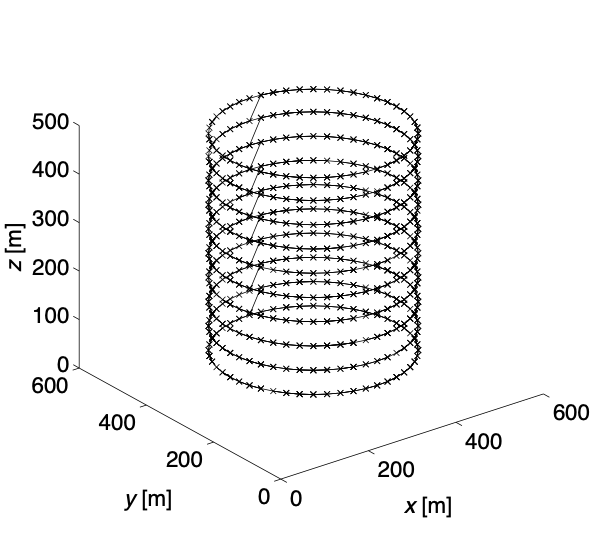
\includegraphics{Fig1.png}
\caption{Write an appropriate figure caption here. Discussions of the implications of the results shown in the figure should be left for the main text. Captions do not end with periods}
\label{fig1}     
\end{figure}


\section{Tables}
Tables should be clearly presented, easy to read, and should be numbered sequentially. Variables presented in the tables should be formatted in the same manner as in the text (e.g., Italic variables and Bold vectors). Each table should include a preceding caption. Tables should be cited as ``Table 1", e.g., ``Table 1 shows ..." or ``the sensible heat flux values are presented in Table 1". If tables are included in the appendices, then these tables should be numbered sequentially continuing from the last table in the main text. Limit the number of tables to five.

\begin{table}
\caption{Write an appropriate caption for the table here. Captions do not end with periods}
\label{tab:1}       
\begin{tabular}{lll}
\hline\noalign{\smallskip}
Variable & Number & Date  \\
\noalign{\smallskip}\hline\noalign{\smallskip}
\textit{x} & 1 & 15/05/2019 \\
\textit{y} & 2 & 16/05/2019 \\
\textit{z} & 3 & 17/05/2019 \\
\noalign{\smallskip}\hline
\end{tabular}
\end{table}


\section{Reference Formatting}
References should be presented in alphabetical order (not in the order of their appearance in the text). They should not be numbered. The total number of pages is not required for book references. List all authors (editors) of referred publications. References can be entered manually using the bibitem structure, or through BibTex (recommended). BibTex users should use the spbasic bibliography style and the natbib package. Sample references of several types are shown below: a journal article \citep{Mason+1987}, a book \citep{Garratt1994}, a book chapter \citep{Wyngaard2004}, a dissertation \citep{Fedorovich1986,Salesky2014}, a technical report \citep{Newsom++2015}, and a paper in conference proceedings \citep{Kaimal1979,Batchvarova+2003, Marusic++2011}.


\begin{acknowledgements}
These should follow the concluding section of the paper and precede the References and any appendices, if they are present. The acknowledgements section does not require a section number. 
\end{acknowledgements} 

\section*{Appendix 1: Title of Appendix}
\{Appendices are optional, as are appendix titles\}\\
Appendices should precede the references and should be numbered (if there is more than one appendix). Equations, tables, and figures contained within the appendices should be numbered sequentially following those in the main text.





\bibliographystyle{spbasic_updated}     
\bibliography{sample_library} 

\newpage

\section*{Supplementary Material for \textit{Boundary-Layer Meteorology} Sample Paper: Instructions for Authors}

{\textbf{First Author* $\cdot$ Second Author $\cdot$ Third Author \\}}
\\
\text{*}Affiliation and email address for the corresponding author only (note that the corresponding author does not need to be the first author).

\section*{1 Supplementary Electronic Materials}
Supplementary multimedia files and other supplementary materials are also accepted for online publication in \textit{Boundary-Layer Meteorology }alongside an article. The supplementary files should be provided in standard file formats.

To accommodate user downloads, please keep in mind that larger-sized files may require very long download times and that some users may experience other problems during downloading.

\subsection*{1.1 Audio, Video, and Animations}
Video and animation files should be provided at an aspect ratio of 16:9 or 4:3. The maximum file size that can be accommodated is 25 GB. The minimum allowable video length is 1 s. The supported file formats include avi, wmv, mp4, mov, m2p, mp2, mpg, mpeg, flv, mxf, mts, m4v, and 3gp. Video files should not contain more than three flashes per second.

\subsection*{1.2 Presentations, Text Files, and Spreadsheets}
Supplemental text files and presentations should be submitted as pdf files. Files in doc or ppt format cannot be accepted. Spreadsheets should also be converted to pdf format if they are intended for viewing only. If readers are encouraged to download and use the spreadsheet, then it can be provided in xls format.

\subsection*{1.3 Specialized Formats}
Other specialized file formats can also be supplied (e.g., tex, pdb, wrl, nb). It is also possible to provide multiple files within a zip or gz file.

\section*{2 General Information}
All supplementary materials should be specifically cited within the main text of the manuscript, in a manner similar to citing tables and figures. The supplementary materials should be cited as ``Online Resource", e.g., ``... as shown in the animation (Online Resource 3)", ``... additional data are provided in Online Resource 4". If more than one supplementary file is provided, these files should be numbered sequentially following the order they are cited in the main text, e.g., ``ESM\_1.mpg", ``ESM\_2.avi". Each supplementary file also requires a concise caption that describes the contents of the file. These captions should be listed at the end of the manuscript at initial submission.

Authors should note that supplementary materials will be published without any conversion, editing, or reformatting. 
\clearpage

\section*{Journal Abbreviations used in \textit{Boundary-Layer Meteorology}}


\begin{longtable}{| p{8 cm} | p{6 cm} |}
\hline
Journal Name & Abbreviation used in BLM \\
\hline
ACM Transactions of Mathematical Software & ACM Trans Math Soft \\
Acoustics Australia & Acoust Aust \\
Acta Geophysica & Acta Geophys \\
Acta Mechanica Synica & Acta Mech Sinica \\
Acta Mechanica Supplement & Acta Mech Suppl \\
Advances in Atmospheric Science & Adv Atmos Sci \\
Advances in Ecological Research & Adv Ecol Res \\
Advances in Meteorology & Adv Meteorol \\
Advances in Science and Research & Adv Sci Res \\
Advances in Water Resources & Adv Water Resour \\
Aeolian Research & Aeolian Res \\
Aerospace Science and Technology & Aerosp Sci Technol \\
Agricultural Meteorology & Agric Meteorol \\
Agricultural and Forest Meteorology & Agric For Meteorol \\
Agricultural Water Management & Agric Water Manag \\
American Institute of Aeronautics and Astronautics & Am Inst Aeronaut Astronaut \\
Annals of Glaciology & Ann Glaciol \\
Annalen der Meteorologie & Ann Meteorol \\
Annals of Statistics & Ann Stat \\
Antarctic Science & Antarct Sci \\
Annual Review of Fluid Mechanics & Annu Rev Fluid Mech \\
Applied Energy & Appl Energy \\
Applied Mechanics Review & Appl Mech Rev \\
Applied Numerical Mathematics & Appl Numer Math \\
Applied Physics B & Appl Phys B \\
Applied Optics & Appl Opt \\
Aquatic Botany & Aquat Bot \\
Archiv f\"{u}r Meteorologie Geophysik und Bioklimatologie Serie A-Meteorologie und Geophysik & Arch Meteorol Geophys Bioklim Ser A \\
Archiv fur Hydrobiologie & Arch Hydrobiol \\
Artificial Intelligence & Artif Intell \\
Astronomy \& Astrophysics & Astron Astrophys \\
Atmospheric Measurement Techniques & Atmos Meas Tech \\
Atmosphere-Ocean & Atmos-Ocean \\
Atmospheric Research & Atmos Res \\
Atmospheric Science Letters & Atmos Sci Lett \\
Australian Journal of Physics & Aust J Phys \\
Australian Journal of Botany & Aust J Bot \\
\hline
Beitraege zur Physik der Atmosphaere & Beitr Phys Atmos \\
Biogeosciences & Biogeosciences \\
Biometrika & Biometrika \\
Biosystems Engineering & Biosyst Eng \\

\hline
\end{longtable}
\newpage

\begin{longtable}{| p{8 cm} | p{6 cm} |}
\hline
Journal Name & Abbreviation used in BLM \\
\hline
Boreal Environment Research & Boreal Environ Res \\
Boundary-Layer Meteorology & Boundary-Layer Meteorol \\
Building and Environment & Build Environ \\
Bulletin of the American Meteorological Society & Bull Am Meteorol Soc \\
\hline
Climate Research & Clim Res \\
Cold Regions Science and Technology & Cold Reg Sci Technol \\
Communications in Agricultural and Applied Biological Sciences & Commun Agric Appl Biol Sci \\
Communications in Mathematical Physics & Commun Math Phys \\
Communications on Pure and Applied Mathematics & Commun Pure Appl Math \\
Comptes Rendus Physique & C R Phys \\
Computers and Electronics in Agriculture & Comput Electron Agric \\
Computing and Informatics & Comput Inf \\
Computer Methods in Applied Mechanical Engineering & Comput Methods Appl Mech Eng \\
Computational Statistics and Data Analysis & Comput Stat Data Anal \\
Contributions to Atmospheric Physics & Contr Atmos Phys \\
Crop Protection & Crop Prot \\
\hline
Deep Sea Research Part II & Deep Sea Res II \\
Dynamics of Atmpsheres and Oceans & Dyn Atmos Oceans \\
\hline
Earth System Science Data Discussions & Earth Syst Sci Data Discuss \\
Earth Surface Processes and Landforms & Earth Surf Process Landf \\
Ecological Applications & Ecol Appl \\
Ecological Indicators & Ecol Indic \\
Ecological Modelling & Ecol Model \\
Ecology & Ecology \\
Electronic Journal of Operational Meteorology & Electron J Oper Meteorol \\
Energies & Energies \\
Energy and Buildings & Energy Buil \\
Energy Conversion and Management & Energy Convers Manag \\
Environmental Fluid Mechanics & Environ Fluid Mech \\
Environmental Modelling and Software & Environ Modell Softw \\
Environmental Pollution & Environ Pollut \\
Environmental Research Letters & Environ Res Lett \\
Environmental Science and Technology & Environ Sci Technol \\
Environmental Software & Environ Softw \\

Eos, Transactions, American Geophysical Union & Eos Trans AGU \\
European Journal of Forest Research & Eur J For Res \\
Experiments in Fluids & Exp Fluids \\
\hline
Fisheries Research & Fish Res \\
Flow Turbulence and Combustion & Flow Turbul Combust \\
Forestry & Forestry \\
Freshwater Biology & Freshwater Biol \\
\hline
\end{longtable}

\pagebreak[4]

\begin{longtable}{| p{8 cm} | p{6 cm} |}
\hline
Journal Name & Abbreviation used in BLM \\
\hline
Functional Ecology & Funct Ecol \\
\hline
Acta Geodaetica et Geophysica Hungarica & Geod Geophys \\
Geografiska Annaler Series A & Geogr Ann Ser A \\
Geography Compass & Geogr Compass \\
Geomorphology & Geomorphology \\
Geophysical Research Letters & Geophys Res Lett \\
Geoscientific Instrumentation, Methods and Data Systems & Geosci Instrum Method Data Syst \\
Geoscientific Model Development & Geosci Model Dev \\
Global Biogeochemical Sciences & Glob Biogeochem Cycles \\
Global Change Biology & Glob Change Biol \\
\hline
Hydrology and Earth System Sciences & Hydrol Earth Syst Sci \\
Hydrological Processes & Hydrol Proc \\
\hline
IEEE Journal of Ocean Engineering & IEEE J Ocean Eng \\
IEEE Transactions on Geoscience and Remote Sensing & IEEE Trans Geosci Remote \\
International Journal of Climatology & Int J Climatol \\
International Journal of Wildland Fire & Int J Wildland Fire \\
International Journal of Heat and Fluid Flow & Int J Heat Fluid Flow \\
International Journal of Numerical Methods for Fluids & Int J Numer Methods Fluids \\
International Journal of Remote Sensing & Int J Remote Sens \\
Izvestiya, Atmospheric and Oceanic Physics & Izv Atmos Ocean Phys \\
\hline
Journal of Advances in Modeling Earth Systems & J Adv Model Earth Syst \\
Journal of Aerosol Science & J Aerosol Sci \\
Journal of Agricultural Engineering Research & J Agric Eng Res \\
Journal of the Air Pollution Control Association & J Air Pollut Control Assoc \\
Journal of Aircraft & J Aircr \\
Journal of Applied Meteorology and Climatology & J Appl Meteorol Clim \\
Journal of Applied Meteorology & J Appl Meteorol \\
Journal of Aquatic Plant Management & J Aquat Plant Manag \\
Journal of Arid Environments & J Arid Environ \\
Journal of Atmospheric and Oceanic Technology & J Atmos Ocean Technol \\
Journal of Atmospheric Science & J Atmos Sci \\
Journal of Climate & J Clim \\
Journal of Computational Physics & J Comput Phys \\
Journal of Earth Simulation & J Earth Simul \\
Journal of Earth System Science & J Earth Syst Sci \\
Journal of Environmental Engineering & J Environ Eng \\
Journal of Experimental Botany & J Exp Bot \\
Journal of the Faculty of Science Hokkaido University & J Fac Sci Hokkaido Univ \\
\hline
\end{longtable}

\pagebreak[4]

\begin{longtable}{| p{8 cm} | p{6 cm} |}
\hline
Journal Name & Abbreviation used in BLM \\
\hline

Journal of Field Robotics & J Field Robot \\
Journal of Fluid Mechanics & J Fluid Mech \\
Journal of Geophysical Research & J Geophys Res \\
Journal of Geophysical Research-Atmospheres & J Geophys Res Atmos \\
Journal of Glaciology & J Glaciol \\
Journal of Great Lakes Research & J Great Lakes Res \\
Journal of Hazardous Materials & J Hazard Mater A \\
Journal of Heat Transfer & J Heat Transf \\
Journal of Hydraulic Engineering & J Hydraul Eng \\
Journal of Hydrology & J Hydrol \\
Journal of Hydrometeorology & J Hydrometeorol \\
Journal of Marine Research & J Mar Res \\
Journal of Marine Systems & J Mar Syst \\
Journal de Mathematiques Pures et Appliquees & J Math Pures Appl \\
Journal of Meteorology & J Meteorol \\
Journal of the Meteorological Society of Japan & J Meteorol Soc Jpn \\
Journal of Oceanography & J Oceanogr \\
Journal of Operational Oceanography & J Oper Oceanogr \\
Journal of the operational Research Society & J Oper Res Soc \\
Journal of the Optical Society of America & J Opt Soc Am \\
Journal of Plankton Research & J Plankton Res \\
Journal of Solar Energy Engineering & J Sol Energy Eng \\
Journal of Quantitative Spectroscopy and Radiative Transfer & J Quant Spectrosc Radiat Transf \\
Journal of Renewable and Sustainable Energy & J Renew Sust Energy \\
Journal of Scientific Statistical Computing & J Sci Stat Comput \\
Journal of Statistical Physics & J Stat Phys \\
Journal of Thermophysics and Heat Transfer & J Thermophys Heat Transf \\
Journal of Tropical Ecology & J Trop Ecol \\
Journal of Turbulence & J Turbul \\
Journal of Wind Engineering and Industrial Aerodynamics & J Wind Eng Ind Aerodyn \\
\hline
Landscape and Urban Planning & Landsc Urban Plan \\
Limnology and Oceanography & Limnol Oceanogr \\
Low Temperature Science & Low Temp Sci \\
\hline
Machine Learning & Mach Learn \\
Marine Chemistry & Mar Chem \\
Mathematische Annalen & Math Ann \\
Meteorological Applications & Meteorol Appl \\
Meteorology and Atmospheric Physics & Meteorol Atmos Phys \\
Meteorologische Zeitschrift & Meteorol Z \\
Monthly Weather Review & Mon Weather Rev \\
\hline
Natural Hazards and Earth System Sciences & Nat Hazards Earth Syst Sci \\
\hline
\end{longtable}

\pagebreak[4]

\begin{longtable}{| p{8 cm} | p{6 cm} |}
\hline
Journal Name & Abbreviation used in BLM \\
\hline
Nature Climate Change & Nat Clim Change \\
Nature Letters & Nat Lett \\
Nature Geoscience & Nat Geosci \\
Neural Computation & Neural Comput \\
Nonlinear Processes in Geophysics & Nonlin Process Geophys \\
New Zealand Journal of Science & N Z J Sci \\
\hline
Oceanography & Oceanography \\
Ocean Dynamics & Ocean Dyn \\
Ocean Engineering Science & Ocean Eng Sci \\
Ocean Modeling & Ocean Model \\
\hline
Papers in Physical Oceanography and Meteorology & Pap Phys Oceanogr Meteorol \\
Particle \& Particle Systems Characterization & Part Part Syst Charact \\
Particuology & Particuology \\
Philosophical Transactions of the Royal Society of London & Philos Trans R Soc \\
Photogrammetric Engineering and Remote Sensing & Photogramm Eng Remote Sens \\
Physical Review Letters & Phys Rev Lett \\
Physical Review E & Phys Rev E \\
Physics and Chemistry of the Earth & Phys Chem Earth \\
Physics of Fluids & Phys Fluids \\
Physics A - Statistical Mechanics and its Applications & Physica A Stat Mech Appl \\
Physica D & Physica D \\
Plant Biosystems & Plant Biosyst \\
PLOS One & PLOS One \\
Powder technology & Powder Technol \\
Proceedings of the Royal Society & Proc Roy Soc \\
Progress in Aerospace Science & Prog Aerosp Sci \\
Progress in Heat and Mass Transfer & Prog Heat Mass Transf \\
Progress in Physical Geography & Prog Phys Geogr \\
Pure and Applied Geophysics & Pure Appl Geophys \\
\hline
Quarterly Journal of the Royal Meteorological Society & Q J R Meteorol Soc \\
\hline
Remote Sensing & Remote Sens \\
Remote Sensing of Environment & Remote Sens Environ \\
Renewable Energy & Renew Energy \\
Reviews of Geophysics & Rev Geophys \\
Reviews of Geophysics and Space Physics & Rev Geophys Space Phys \\
Review of Scientific Instruments & Rev Sci Inst \\
\hline
Science & Science \\
Science of the Total Environment & Sci Tot Environ \\
Sedimentology & Sedimentol \\
Siam Journal on Applied Mathematics & SIAM J Appl Math \\
\hline
\end{longtable}

\pagebreak[4]

\begin{longtable}{| p{8 cm} | p{6 cm} |}
\hline
Journal Name & Abbreviation used in BLM \\
\hline
Tellus & Tellus \\
Tellus Series B - Chemical and Physical Meteorology & Tellus Ser B Chem Phys Meteorol \\
Theoretical and Applied Climatology & Theor Appl Climatol \\
Theoretical and Computational Fluid Dynamics & Theor Comput Fluid Dyn \\
Theoretical Computational Fluid Dynamics & Theor Comput Fluid Mech \\
Thermal Science Engineering & Therm Sci Eng \\
Transactions of the American Society of Agricultural Engineers & Trans ASAE \\
Tree Physiology & Tree Physiol \\
Trudy Geofizicheskogo Instituta, Akademiya Nauk SSSR & Trudy Geofiz Inst AN SSSR \\
\hline
Urban Climate & Urban Clim \\
\hline
Water Air and Soil Pollution & Water Air Soil Pollut \\
Water Resources Research & Water Resour Res \\
Waterway Port Coastal and Ocean Engineering & Waterw Port Coast Ocean Eng \\
Weather & Weather \\
Weather and Forecasting & Weather Forecast \\
Wind Energy & Wind Energy \\
Wind Engineering & Wind Eng \\
\hline
Zeitschrift f\"{u}r Angewandte Mathematik und Mechanik & Z Agnew Math Mech \\
\hline



\hline
\end{longtable}

\end{document}

